\textcolor{blue}{Problem 1}
Referring to Figure 4.10, why are both curves increasing with $K$? Why do they converge to each other with increasing $K$? (20pt)
\begin{figure}[htbp]
    \centering
    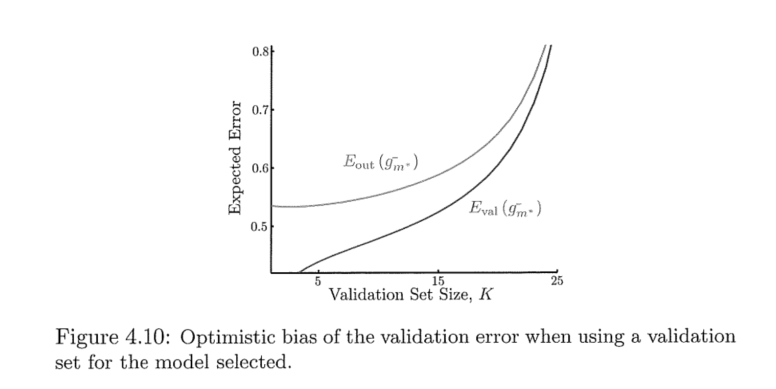
\includegraphics[width=1.0\textwidth]{../fig/figure.png}
\end{figure}
\par


\textcolor{blue}{Solution}\\
1. Since the size of the total data is fixed, so as $K$ increases, there are less points used for training. We can assume that are data points are useful data, so less data points used for training will lead to a worse model. And it is reasonable that the performence of the model both on training set and validation set will decrease. i.e. they all have a larger expected error.

So above all, as $K$ increases, the both curves increase.\\

2. From what we have learned, we can get that
$$E_{\text{out}}(g^-_{m^*})\leq E_{\text{val}}(g^-_{m^*})+O\left(\sqrt{\frac{\ln M}{K}}\right)$$
Where $M=\mathcal{H}_{\text{val}}$, $K$ is the size of validation set.\\
Since $M$ is fixed, so the difference between $E_{\text{out}}(g^-_{m^*})$ and $E_{\text{val}}(g^-_{m^*})$ is $O\left(\sqrt{\frac{\ln M}{K}}\right)$, which decreases as $K$ increases.\\

So above all, as $K$ increases, the difference of the two curves decreases, and they converge to each other.

\newpage